%\packagelist
\documentclass{article}
\usepackage[top=3cm, bottom=3cm, outer=3cm, inner=3cm]{geometry}
\usepackage{multicol}
\usepackage{graphicx}
\graphicspath{{img/}}
\usepackage{url}
%\usepackage{cite}
\usepackage{hyperref}
\usepackage{array}
%\usepackage{multicol}
\newcolumntype{x}[1]{>{\centering\arraybackslash\hspace{0pt}}p{#1}}
\usepackage{natbib}
\usepackage{pdfpages}
\usepackage{multirow}
\usepackage[normalem]{ulem}
\useunder{\uline}{\ul}{}
\usepackage{svg}
\usepackage{xcolor}
\usepackage{listings}
\lstset{basicstyle=\ttfamily,
  showstringspaces=false,
  commentstyle=\color{red},
  keywordstyle=\color{blue}
}
%\usepackage{booktabs}
\usepackage{caption}
\usepackage{subcaption}
\usepackage{float}
\usepackage{array}

\newcolumntype{M}[1]{>{\centering\arraybackslash}m{#1}}
\newcolumntype{N}{@{}m{0pt}@{}}


%%%%%%%%%%%%%%%%%%%%%%%%%%%%%%%%%%%%%%%%%%%%%%%%%%%%%%%%%%%%%%%%%%%%%%%%%%%%
%%%%%%%%%%%%%%%%%%%%%%%%%%%%%%%%%%%%%%%%%%%%%%%%%%%%%%%%%%%%%%%%%%%%%%%%%%%%
\newcommand{\itemEmail}{lsequeiros@unsa.edu.pe}
\newcommand{\itemStudent}{Luis Gustavo Sequeiros Condori}
\newcommand{\itemCourse}{Programación Web I}
\newcommand{\itemSemester}{II}
\newcommand{\itemUniversity}{Universidad Nacional de San Agustín de Arequipa}
\newcommand{\itemFaculty}{Facultad de Ingeniería de Producción y Servicios}
\newcommand{\itemDepartment}{Departamento Académico de Ingeniería de Sistemas e Informática}
\newcommand{\itemSchool}{Escuela Profesional de Ingeniería de Sistemas}
\newcommand{\itemAcademic}{2023 - B}
\newcommand{\itemInput}{Del 6 Enero 2024}
\newcommand{\itemOutput}{Al 10 Enero 2024}
\newcommand{\itemPracticeNumber}{11}
\newcommand{\itemTheme}{JavaScript}
%%%%%%%%%%%%%%%%%%%%%%%%%%%%%%%%%%%%%%%%%%%%%%%%%%%%%%%%%%%%%%%%%%%%%%%%%%%%
%%%%%%%%%%%%%%%%%%%%%%%%%%%%%%%%%%%%%%%%%%%%%%%%%%%%%%%%%%%%%%%%%%%%%%%%%%%%

\usepackage[english,spanish]{babel}
\usepackage[utf8]{inputenc}
\AtBeginDocument{\selectlanguage{spanish}}
\renewcommand{\figurename}{Figura}
\renewcommand{\refname}{Referencias}
\renewcommand{\tablename}{Tabla} %esto no funciona cuando se usa babel
\AtBeginDocument{%
	\renewcommand\tablename{Tabla}
}

\usepackage{fancyhdr}
\pagestyle{fancy}
\fancyhf{}
\setlength{\headheight}{30pt}
\renewcommand{\headrulewidth}{1pt}
\renewcommand{\footrulewidth}{1pt}
\fancyhead[L]{\raisebox{-0.2\height}{
\includegraphics[width=3cm]{logo_episunsa.png}}}
\fancyhead[C]{\fontsize{7}{7}\selectfont	\itemUniversity \\ \itemFaculty \\ \itemDepartment \\ \itemSchool \\ \textbf{\itemCourse}}
\fancyhead[R]{\raisebox{-0.2\height}{
\includegraphics[width=1.2cm]{logo_abet.png}}}
\fancyfoot[R]{Página \thepage}

% para el codigo fuente
\usepackage{listings}
\usepackage{color, colortbl}
\definecolor{numberOrange}{RGB}{235, 126, 9}
\definecolor{mygreen}{RGB}{40, 194, 6}
\definecolor{dkgreen}{rgb}{0,0.6,0}
\definecolor{myblue}{RGB}{57, 118, 189}
\definecolor{gray}{rgb}{0.156,0.146,0.135}
\definecolor{mygray}{RGB}{135, 135, 135}
\definecolor{mauve}{rgb}{0.58,0,0.82}
\definecolor{codebackgroundCode}{RGB}{10, 10, 20}
\definecolor{codebackgroundBash}{rgb}{0.95, 0.95, 0.92}
\definecolor{tablebackground}{RGB}{10, 25, 115}
\definecolor{lines}{RGB}{0, 120, 250}

\arrayrulecolor{lines}
\lstdefinestyle{custom}{
  %Las líneas que encierran al código: top, below, left, right. COn mayúsculas son dos líneas
  frame=tlrb,
  %Los espacios en los strings s muestran con normalidad, no con carácter especial
  showstringspaces=false,
  %no tiene cuidado del alineamiento de columnas, contrario a fixed, con ese valor es más riguroso
  columns=flexible,
  %Permite saltos de línea cuando el texto es muy largo
  breaklines=true,
  %Luego de un salto de línea automático, se coloca una flecita roja
  postbreak=\mbox{\textcolor{red}{$\hookrightarrow$}\space},
  %Los saltos de línea solo deben ocurrir en espacios en blanco
  breakatwhitespace=true,
  %espacios de tabulador
  tabsize=2,
  %No mostrar tabulador como caracter, como un espacio y ya
  showtabs=false,
  %No mostrar los espacios como caracteres
  showspaces=false,
  %No mostrar líneas al final de los listados
  showlines=false,
  %La codificación del archivo
  inputencoding=utf8,
  %Permite manejar los caracteres especiales junto con inputencoding  el paquete inputenc
  extendedchars=true,
  %
  literate={á}{\'a}1 {é}{\'e}1 {í}{\'i}1 {ó}{\'o}1 {ú}{\'u}1 {¿}{\textquestiondown}1 {ñ}{\~n}1 {Ñ}{\~N}1 
  {Á}{\'A}1 {É}{\'E}1 {Í}{\'I}1 {Ó}{\'O}1 {Ú}{\'U}1 {¡}{\textexclamdown}1
}

\lstdefinestyle{perl}{
  style=custom,
	language=Perl,
	basicstyle={\footnotesize\ttfamily\color[RGB]{255,255,255}},
	numberstyle=\color{mygray},
	numbers=left, 
  framexleftmargin=8mm,
  framexrightmargin=8mm,
  keywordstyle={\color{myblue}\itshape},
	%morekeywords={String, System, List, ArrayList, LinkedList, Scanner, Map, HashMap, TreeMap, Scanner},
  commentstyle={\color{mygray}\itshape},
  identifierstyle=\color[RGB]{16,151,228},
	stringstyle=\color{mygreen},
  %emph={int, char, boolean, String, double, float, byte, long, short, Integer, Character, Soldado, Boolean, Double, Float, Byte, Long, Short, List, Scanner, Map},
  emphstyle={\color[RGB]{244,151,32}},
	backgroundcolor= \color{codebackgroundCode}
}
\lstdefinestyle{html}{
  style=custom,
  language=HTML,
	basicstyle={\footnotesize\ttfamily\color[RGB]{255,255,255}},
	numberstyle=\color{mygray},
	numbers=left, 
  framexleftmargin=8mm,
  framexrightmargin=8mm,
  keywordstyle={\color{myblue}\itshape},
	%morekeywords={String, System, List, ArrayList, LinkedList, Scanner, Map, HashMap, TreeMap, Scanner},
  commentstyle={\color{mygray}\itshape},
  identifierstyle=\color[RGB]{16,151,228},
	stringstyle=\color{mygreen},
  %emph={int, char, boolean, String, double, float, byte, long, short, Integer, Character, Soldado, Boolean, Double, Float, Byte, Long, Short, List, Scanner, Map},
  %emphstyle={\color[RGB]{244,151,32}},
	backgroundcolor= \color{codebackgroundCode}
}
\lstdefinestyle{css}{
  style=custom,
  language=CSS,
	basicstyle={\footnotesize\ttfamily\color[RGB]{255,255,255}},
	numberstyle=\color{mygray},
	numbers=left, 
  framexleftmargin=8mm,
  framexrightmargin=8mm,
  keywordstyle={\color{myblue}\itshape},
	%morekeywords={String, System, List, ArrayList, LinkedList, Scanner, Map, HashMap, TreeMap, Scanner},
  commentstyle={\color{mygray}\itshape},
  identifierstyle=\color[RGB]{16,151,228},
	stringstyle=\color{mygreen},
  %emph={int, char, boolean, String, double, float, byte, long, short, Integer, Character, Soldado, Boolean, Double, Float, Byte, Long, Short, List, Scanner, Map},
  %emphstyle={\color[RGB]{244,151,32}},
	backgroundcolor= \color{codebackgroundCode}
}
\lstdefinestyle{mybash}{
  style=custom,
	language=bash,
	keepspaces=true,
	basicstyle={\small\ttfamily},
	keywordstyle=\color{myblue},
	morekeywords={java, javac, git},
	commentstyle=\color{mygray},
	stringstyle=\color{mygreen},
	backgroundcolor= \color{codebackgroundBash}
}

\begin{document}
	
	\vspace*{10px}
	
	\begin{center}	
		\fontsize{17}{17} \textbf{ Informe de Laboratorio \itemPracticeNumber}
	\end{center}
	\centerline{\textbf{\Large Tema: \itemTheme}}
	\vspace*{0.5cm}	

	\begin{table}[H]
		\begin{tabular}{|x{4.7cm}|x{4.8cm}|x{4.8cm}|}
			\hline 
			\rowcolor{tablebackground}
			\color{white} \textbf{Estudiante} & \color{white}\textbf{Escuela}  & \color{white}\textbf{Asignatura}   \\
			\hline 
      {\itemStudent \par \itemEmail} & \itemSchool & {\itemCourse \par Semestre: \itemSemester}     \\
			\hline 			
		\end{tabular}
	\end{table}		
	
	\begin{table}[H]
		\begin{tabular}{|x{4.7cm}|x{4.8cm}|x{4.8cm}|}
			\hline 
			\rowcolor{tablebackground}
			\color{white}\textbf{Semestre académico} & \color{white}\textbf{Fecha de inicio}  & \color{white}\textbf{Fecha de entrega}   \\
			\hline 
			\itemAcademic & \itemInput &  \itemOutput  \\
			\hline 
		\end{tabular}
	\end{table}

	\section{Objetivos}
	\begin{itemize}		
    \item Conocer el lenguaje JavaScript
	\end{itemize}
		
	\section{Temas a Tratar:}
	\begin{itemize}
		\item JavaScript
	\end{itemize}
	
	\section{JavaScript}

  \subsection{¿Qué puede hacer?}

 \begin{itemize}
   \item Cambiar el contenido HTML
   \item Cambiar los atributos HTML
   \item Cambiar los estilos de los elementos HTML
   \item Esconder y mostrar elementos HTML
 \end{itemize}

 \subsection{¿Dónde está?}
 \begin{itemize}
   \item Puede ser insertado en la etiqueta <script>, pueden estar situados en body o head.
   \item Situar los scripts debajo de los elementos mejora la visualización, la interpretación del script hace más lenta la página.
   \item También puede estar situado en archivos externos, con\lstinline{<script src="file.js></script>}
   \item Se comportará de acuerdo a donde esté ubicado la etiqueta <script>
   \item Los scripts externos no pueden contener etiquetas <script>
   \item Con scripts externos, el programa es fácil de modificar y de leer
   \item El almacenamiento en caché puede acelerar la carga de la página
 \end{itemize}

 \subsection{La salida}
 \begin{itemize}
   \item Puede escribir en un elemento HTML, en la salida HTML, en una ventana de alerta o en la consola del navegador
   \item innerHTML: Cambia el contenido de la etiqueta. \lstinline{document.getElementById("demo").innerHTML = 5 + 6;}
   \item document.write() puede ser utilizado con fines de testeo. Cuando se usa document.write() luego de haber cargado la página, esta borrará su contenido y se escribirá lo ingresado (sobreescribir)
   \item window.alert(), se utiliza para mostrar datos. Se puede skipear el objeto window, ya que tiene alcance global. Eso significa que todas las variables y métodos pertenecen al objeto window.
   \item console.log() para propósitos de debugeo, muestra la salida en la consola del navegador
   \item window.print(), imprime (abre una ventana para imprimir en impresora) el contenido de la ventana actual.
 \end{itemize}

 \subsection{Sentencias}

 \begin{itemize}
   \item  Las sentencias de JavaScript son ejecutadas por el navegador
   \item Se componen de valores, operadores, expresiones, claves y comentarios
   \item Se ejecutan una a una en el orden en el que están escritos
   \item Al final de una sentencia se debe colocar punto y coma (semicolon), no es obligatorio pero si muy recomendable
   \item Una buena práctica es que la línea no tenga más de 80 caracteres, asimismo, el meor lugar para romper una línea es después de un opereador
   \item Las sentencias pueden ser agrupadas en bloques delimitados por llaves.
   \item A menudo las sentencias inician con una palabra clave para indicar la acción a realizar
 \end{itemize}

 \begin{figure}[H]
   \centering
   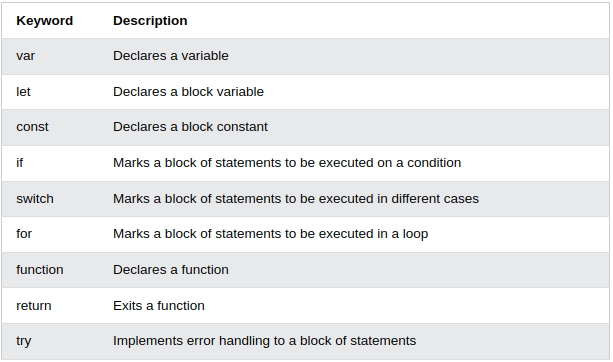
\includegraphics[width=0.6\textwidth]{img/table1.png}
   \caption{Palabras clave en JS}
 \end{figure}

 \subsection{Sintaxis}

 \begin{itemize}
   \item Hay dos tipos de valores: fijos(literales) y variables
   \item  Literales: Lo números son escritos con o sin decimales, Strings con comillas dobles o simples
   \item Variables: Almacenan valores. Las claves var, let y const declaran variables.
   \item El signo = asigna valores
   \item Operadores: + -  /
   \item Expresiones: Una combinación de variables, valores y operadores, con los que se calcula un valor. El cálculo es llamado Evaluación
   \item Comentarios: Luego de // o entre /* */
   \item Identificadores: Empiezan con letras,\textdollar o _, no con números. Distinguen entre mayúsculas y minúsculas.
   \item Utiliza Unicode
 \end{itemize}

 \subsection{Variables}

 \begin{itemize}
   \item Se pueden declara de 4 formas: Automáticamente, var, let y const (se considera buena práctica declarar las variables antes de usarlas)
   \item var fue usada desde 1995 a 2015 (solo debe ser usada en código escrito para navegadores antiguos)
   \item let y const fueron añadidas en 2015
   \item una variable declarada con let puede ser cambiada, con const no.
   \item const si el valor no debe cambiarse, si el tipo no debe cambiarse (arreglos y objetos)
   \item usar let solo si no se puede usar const
   \item En una declaración, la variable no tiene valor (undefined)
   \item Es una buena práctica declarar todas las variables al inicio del código
   \item Se puede declarar en una línea separando por coma
   \item Si se vuelve a declarar una variable declarada con var, esta no perderá su valor. No se puede redeclarar una varible declarada con let y const
   \item Si en una operación aritmética se encuentra un String, los números siguientes se comportarán como String.
   \item Es una convención utilizar _ al inicio del nombre de una variable "escondida"
 \end{itemize}

 \subsection{Let y const}

 \begin{itemize}
   \item Estas dos le brinda a las variables un ámbito, las variables declaradas con var tienen un ámbito global
   \item Ojo que si se puede "redeclarar" una variable let, per en un ámbito diferente (incluso si es un ámbito hijo y el padre tiene declarada ya la variable)
   \item Las variables const deben ser asignadas al momento de ser declaradas. Definen una referencia constante, no un valor constante.
   \item Usa const cuando declares arreglos, objetos, funciones y regEXP, su valor puede cambiar que la referencia no
 \end{itemize}

 \subsection{Aritmética}

 \begin{figure}[H]
   \centering
   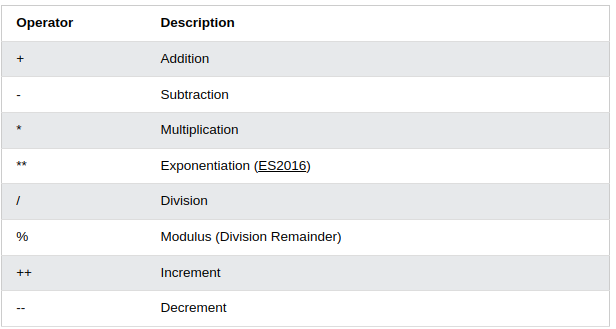
\includegraphics[width=0.6\textwidth]{img/table2.png}
   \caption{Operadores de asignación}
 \end{figure}

 \begin{figure}[H]
   \centering
   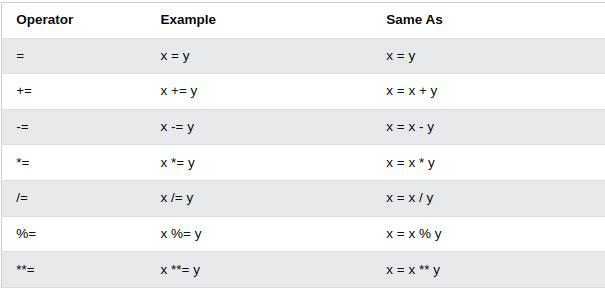
\includegraphics[width=0.6\textwidth]{img/table3.png}
   \caption{Operadores de comparación}
 \end{figure}

 \begin{itemize}
   \item Los strings se comparan alfabeticamente
   \item Cuando se unsa + en Strings es un operador de concatenación
   \item Los operadores lógicos son los mismos que en Java
   \item typeof: devuelve tipo de variable, instanceof: true si es una instancia de un tipo de objeto
 \end{itemize}
 \begin{figure}
   \centering
   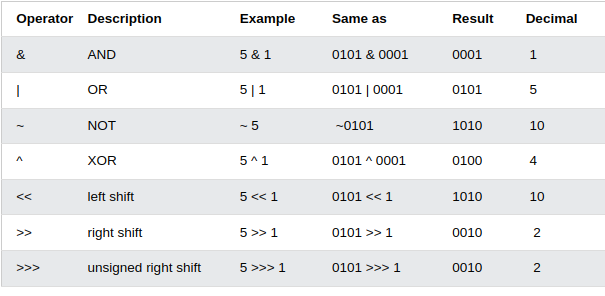
\includegraphics[width=0.6\textwidth]{img/table4.png}
   \caption{Operadores bit a bit}
 \end{figure}
 \begin{itemize}
   \item El operador ** es de potenciación
 \end{itemize}
 \subsection{Tipos de Datos}

 \begin{itemize}
   \item Los tipos son dinámicos, la misma variable puede ser usada para contener diferentes tipos de datos
   \item BigInt() puede ser usado para representar valores más grandes que 64 bit (todas las variables tienen este almacenamiento)
 \end{itemize}

 \subsection{Funciones}

 \begin{itemize}
   \item Bloque de código designado a una tarea en particular
   \item \lstinline{function name(parameter1, parameter2, parameter3)}
   \item En la función , los parámetros  se comportan como variables locales
   \item Se invoca cuando un evento ocurre, invocado por código JS o autoinvocado.
 \item return detiene la función y retorna una valor
 \item Al colocar el nombre de la función sin paréntesis, se la trata como objeto
 \item Las funciones tiene su propio ámbito
 \end{itemize}

 \subsection{Objetos}

 \begin{itemize}
   \item Los objetos también son variables, pero contienen más valores
   \item \lstinline{const car = \{type:"Fiat", model:"500", color:"white"\};}
   \item Los espacios y saltos de línea no son importantes aquí
   \item Para acceder a una propiedad del objeto \lstinline{car.type} o \lstinline{car["type"]}
   \item Los objetos pueden tener métodos, los cuales se tratan como propiedades en estos \lstinline{fullName : function()\{ return this.firstName + " " + this.lastName;\}}
   \item this tiene diferentes significados, en la tabla de abajo se encuentra su explicación
   \item En una definición de función, this se refiere al propietario de la función (objeto que tiene la función)
   \item \lstinline{objectName.methodName()}
   \item No es bueno declarar literales como objetos.
 \end{itemize}

 \subsection{Strings}
 \begin{itemize}
   \item Una cadena de plantilla permite comillas dobles y simples dentro de ella \lstinline{let text = `He's often called "Johnny"`;}
   \item Para el largo de un String se utiliza la propiedad length (como arrayas en Java)
   \item Backslash permite "escapar" caracteres
   \item OJO:Comparar dos objetos en JS siempre retorna false
   \item charAt() devuelve el carácter  de la posición especificada, charCodeAt() devuelve el código del carácter en UTF-16 (un entero)
   \item at(), es lo mismo que chatAt(), funciona desde 2022, admite posiciones negativas
   \item También se puede acceder como si fuera un arreglo, es impredecible, si no encuentra caracter retorna indefinido, charAt retorna un string vacío. Es solo de lectura, no se puede modificar contenido como en un arreglo.
   \item slice(start, end), extrae una parte del string y lo retorna en un nuevo string, si solo se ingresa un parámetro, entonces extrae desde ahí hasta el final del string. Si el parámetro es negativo, cuenta desde atrás
   \item Con substring() pasa algo similar, pero los valores negatios se tratan con 0.
   \item substr(start, length), si el inicio es negativo se cuenta desde atrás
   \item toUpperCase() y toLowerCase(), para mayúsculas y minúsculas.
   \item Los Strings son inmutables
   \item trim() remueve los espacios en blanco a los costados del string. trimStart() los remueve solo del comienzo, trimEnd() del final. (2019)
   \item repeat(n), repite n veces el string
   \item replace(pattern, rep) replaza la primera coincidencia. Si se desea que no se diferencia entre mayúsculas y minúsculas /MICROSOFT/i. Para reemplazar todas las coincidencias se puede usar expresiones regulares /Microsoft/g
   \item replaceAll() funiona con expresiones regulares (2021)
   \item split() devuelve un arreglo a partir de un separador
   \item indexOf() posición de la primera ocurrencia, -1 si no encuentra nada
   \item lastIndexOf() la última ocurrencia
   \item Ambos admiten un segundo parámetro, que es la psición de donde empezará a buscar
   \item search() busca un string o una expresión regular, no tiene un segundo parámetro, indexOf() no acepa expresiones regulares
   \item match() retorna un array que contiene los resultados de las coincidencias. matchAll() devuelve un iterador (2020)
   \item includes() retorna true si contiene un valor específico, Acepta un segundo parámetro de posición
   \item startsWith() y endsWith(), empieza o termina con una cadena
   \item Tempate Strings: Entre comillas invertidas, aceptan multilíneas, acepta la interpolación con \$\{...\}
 \end{itemize}

 \subsection{Números}
 \begin{itemize}
   \item Los números grandes se pueden expresar con notación científica
   \item Todos los números son almacenados como reales flotantes precisos en 64 bits, el número se almacena en los bits del 0 al 51, el exponente del 52 al 62 y el signo en el bit 63
   \item Los números enteros tiene una precisión de hasta 15 dígitos
   \item La aritmétca de la coma flotante no es siempre precisa
   \item JS siempre trata de hacer las operaciones correctas (+,-, /, *) cuando se trata de strings numéricos. Sin embargo, + es un operador de concatenación para strings, por lo suqe no funciona correctamente
   \item NaN es una palabra reservada que indica que el número no es algo admitido. isNan() nos ayuda a determinar este valor
   \item Cualquier operación matemática con NaN será otro NaN
   \item Infinity es el valor que JS devolverá s calcula un número fuera del mayor posible
   \item Hexadecimales, Js interpretanúmeros hexadecimales si están precedidos por 0xFF (nunca escribir un número con 0 a la izquierda ya que algunas versiones lo interpretan como octales)
   \item BigInt es el segundo tipo numérico de dato en JS
   \item Number.MAX_SAFE_INTEGER y Number.MIN_SAFE_INTEGER, Number.EPSILON, Number.MAX_VALUE, Number.MIN_VALUE, Number.POSITIVE_INFINITY, Number.NEGATIVE_INFINITY, Number.NaN 
   \item isInteger() para saber si es un número enteros
   \item toString(), retorna un número como String
   \item toExponential(), retorna un número escrito en su notación exponencial
   \item toFixed(), retorna un número escrito con un número de decimales
   \item toPrecision(), retorna un número con un laro especial
     \item valueOf(), retorna un número como número
     \item De variable a número, Number(), parseFloat() parseInt()
 \end{itemize}

 \subsection{Arreglos}

 \begin{itemize}
   \item \lstinline{const array_name = \[item1, item2, ...\];  }
   \item Espacios y saltos de línea no importan en la declaración del arreglo
   \item El arreglo se pueden inicializar como objeto, pero para más simplicidad es mejor hacerlo como arriba 
   \item Para convertir un arreglo a String simplemente hay que utilizar el método toString()
   \item atributo length para saber su largo, sort() ordena el arreglo
   \item Se puede añadir otro elemento utilizando push(), o también utilizando la propiedad length
   \item No se puede crear un objeto array (con new) con un solo elemento, digamos new Array(3), crea un array de tres elementos indefinidos
   \item Array.isArray() compureba si el elemento es un arreglo o no
   \item at() permite ingresar números negativos para contar las posiciones desde atrás
   \item join() devuelve los elementos del arreglo en String pero divididos pors el parámetro del método
   \item pop() guarda el último elemento y lo quita del arreglo
   \item shift() remueve y guarda primer elemento del arreglo
   \item unshift() añade un nuevo elemento al comienzo
   \item keyword delete borra un elemento, pero deja un espacio en indefinido
   \item concat() concatena dos o más arreglos
   \item splice(start, end) para eliminar elementos sin dejar agujeros en el arreglo
   \item toSpliced() hace lo mismo pero crea una copia del arreglo para no modificar el original
   \item slice() elimina elementos sin modificar el arreglo original
 \end{itemize}

 \subsection{Fecha}

 \begin{figure}[H]
   \centering
   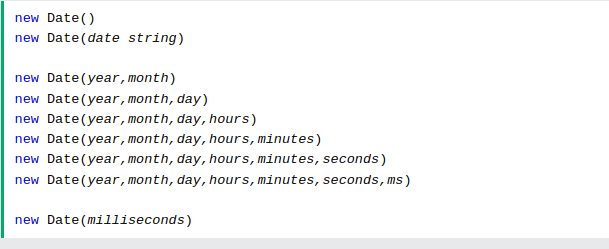
\includegraphics[width=0.6\textwidth]{table5.png}
   \caption{Constructores Date}
 \end{figure}

 \begin{figure}[H]
   \centering
   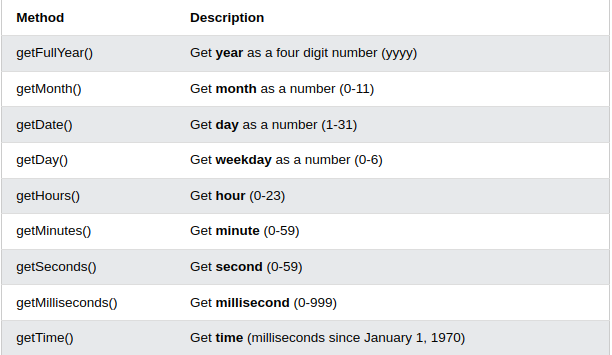
\includegraphics[width=0.6\textwidth]{table6.png}
   \caption{Métodos de get de Date}
 \end{figure}

 \begin{figure}[H]
   \centering
   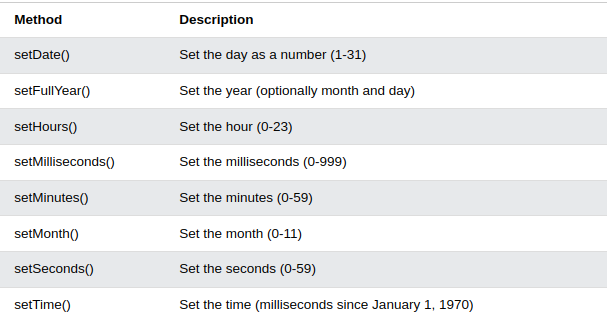
\includegraphics[width=0.6\textwidth]{table7.png}
   \caption{Métodos de set de Date}
 \end{figure}

 \begin{itemize}
   \item Los objetos de fecha son estáticos, no están corriendo
   \item toDateString(), toUTCString(), toISOString()
 \end{itemize}

 \subsection{Math}
 \begin{figure}[H]
   \centering
   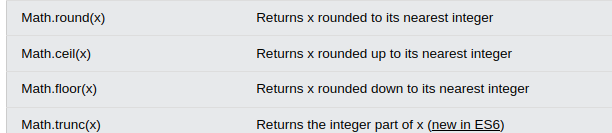
\includegraphics[width=0.6\textwidth]{table8.png}
   \caption{Algunos métodos de Math}
 \end{figure}
 \begin{itemize}
   \item Es un objeto estático, por ello no tiene constructor
   \item Math.random() devuelve un número aleatorio entre 0 y 1
 \end{itemize}

 \subsection{If,else, switch}

 \begin{itemize}
   \item Funcionan tal como en Java
   \item El default del switch no necesariamente tiene que ser el último Bloque
   \item switch utiliza la comparación estricta === (valor y tipo)
 \end{itemize}

 \subsection{Bucles}

 \begin{itemize}
   \item For normal funciona como en Java
   \item For in es utilizado para iterar en las propiedades de un objeto \lstinline{for (key in object)}, también puede servir en arreglos \lstinline{for (variable in array)}
   \item For of es para objetos iterables \lstinline{for (variable of iterable)} arreglos, strings, mapas nodelists, etc
   \item while y do while son lo mismo que en Java
   \item Break puede ayudarnos a salir del Bucles
   \item continue  interrumpe una iteración de acuerdo a un caso específico, continúa con la siguiente iteración
   \item Un label es un conjunto de snetencias con un nombre label: \{sentencias\} , break y continue se pueden utilizar aquí break label; contnue label;
 \end{itemize}

 \subsection{Mapas}

 \begin{figure}[H]
   \centering
   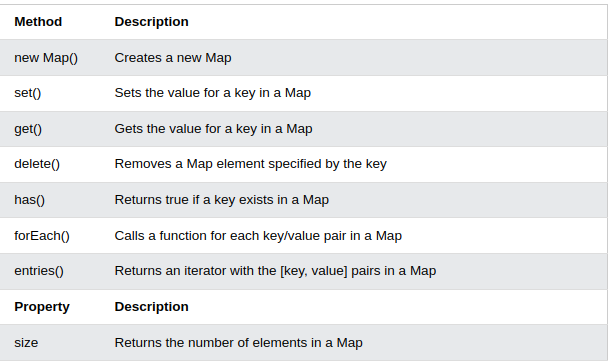
\includegraphics[width=0.6\textwidth]{table9.png}
   \caption{Algunos métodos  de Mapas}
 \end{figure}

 \subsection{Expresiones regulares}

 \begin{itemize}
   \item Modificadores: i, case sensitive; g, encontrar todas las coincidencias; m, con diferentes líneas; d, coincidencia de inicio y final
   \item [abc], [0-9], (x|y) como en perl
   \item \\d para dígito, \\s espacio en blanco , \\b match al inicio o final de la palabra
   \item \\uxxxx encontrar un caracter unicode especial
   \item *, +; ? como el Perl
   \item el objeto expresión regular \lstinline{const pattern = /e/; pattern.test("The best things in life are free!");} retorma true si lo contiene, en esste caso si es true
 \end{itemize}

 \subsection{Errores}
 \begin{itemize}
   \item try catch como en Java, el parámetro de catch es err
   \item El objeto error de  JS tiene dos propiedades, name y message
   \item COn throw puedes crear un error personalizado, para manejarlo luego con try catch
   \item Finally permite ejecutar código después del try catch, independientemente del resultado
 \end{itemize}

 \begin{figure}[H]
   \centering
   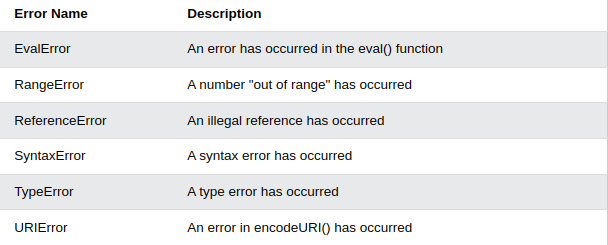
\includegraphics[width=0.6\textwidth]{table10.png}
   \caption{Seis errores de JS}
 \end{figure}

 \subsection{Fetch}
 
  \begin{itemize}
    \item Video sobre el funcionamiento de la página \url{https://youtu.be/6ISN8tj86vQ}.
    \item Repositorio de GitHub para commits \url{https://github.com/gusCreator/pweb-course/tree/main/lab10}.
  \end{itemize}

\clearpage
	
%\clearpage
%\bibliographystyle{apalike}
%\bibliographystyle{IEEEtranN}
%\bibliography{bibliography}
			
\end{document}
